\documentclass[11pt]{book}              % Book class in 11 points
\usepackage[utf8]{inputenc}
\usepackage[english]{babel}
\usepackage{graphicx}
\parskip3pt

\usepackage{caption}
\usepackage{subcaption}

\usepackage{rotating}
% \usepackage{subfig}

% Horizontal overline denoting negation:
\newcommand{\NOT}[1]{$\overline{\mbox{#1}}$}

\title{\bf How to Design \& Build Your Own Custom TV Games}
\author{David L. Heiserman}
\date{November, 1978}

\begin{document}
\frontmatter
\maketitle

\section{Dedication}
This book is dedicated to the growing number of young women who have the motivation and courage to join the ranks of skilled digital electronics technicians and engineers.

\newpage
%
% Other TAB books by the author:
%
% No. 714 Radio Astronomy for the Amateur
% No. 841 Build Your Own Working Robot
% No. 971 Mimbrocessors: From Calculators to Computers
%
% No.1101
% $15.95
%
% How to Design & Build Your Own Custom TV Games
% by David L. Heiserman
%
% TAB TAB BOOKS Inc.
%
% BLUE RIDGE SUMMIT, PA. 17214
%
% FIRST EDITION
%
% FIRST PRINTING — NOVEMBER 1978
% SECOND PRINTING — APRIL1980
% THIRD PRINTING — APRIL 1981
%
% Copyright © 1978 by TAB BOOKS Inc.
% Printed in the United States of America
%
% Reproduction or publication of the content in any manner, without express
% permission of the publisher, is prohibited. No liability is assumed with respect
% to the use of the information herein.
%
% Library of Congress Cataloging in Publication Data
%
% Heiserman. David L. 1940-
% How to design and build your own custom TV games.
%
% includes index.
% 1. Video games - Equipment and supplies - Design and construction — Amateur‘s manuals. I. Title.
% TK9971.H44 688.7’28 78-11389
% ISBN 0-8306-9859-0
% ISBN 0-8306-1101-0 pbk.
%

\section{Preface}

America is a nation accustomed to fads. Novel ideas and products catch on rather quickly, sweeping the country with new products and
services. More often than not, these fads gradually change form or
fade away with time.

TV games had all the earmarks of being one of these fads at
first. Once the idea caught on, video game products captured the fancy of all sorts of people — people willing to put out \$50, \$60 or, in some cases, more than a \$100 to play the fascinating little games in their own homes.

But it appears that TV games are here to stay. The games are becoming more sophisticated and diverse, and product sales skyrocket every Christmas. What’s more, commercial, coin-operated versions have already transformed the game arcade industry into something totally new and different. It now seems that video games are replacing the pinball machine as America’s number-one arcade game.

This is a book about TV games. It shows how they work and, more importantly, how to design and build custom versions. This book is not merely a collection of complete TV game circuits. To be sure, there are a number of complete game circuits presented as design examples; the real emphasis is on designing and building custom TV games. In fact the reader will loose much of the fun of the whole thing by simply copying the circuits shown here.

The whole idea of the book is to release the reader’s creative instincts, transforming them into custom games that are a delight to the designer as well as others who have an opportunity to enjoy them.

The game systems as they are presented here might seem rather cumbersome compared to the slick, cassette-programmed game systems on the market today. But how creative can one be with someone else’s prescribed programs? Sure it is possible to get a dozen games on one program tape, but it really doesn’t take long to want more. The game-design scheme presented in this book is wholly open-ended — there is no real limit to the number and types of games that can come from it. It’s all a matter of learning how to design the games and exercising some degree of creativity and imagination.

It is not necessary to have a great deal of know-how concerning digital electronics to begin the work in this book. The first few chapters have been planned with the digital novice in mind. As the work progresses, however, the need for learning more about basic digital electronics becomes more apparent. Unfortunately, a book of this size cannot stand up as both a design manual for video games and a text book on basic digital electronics.

While the information regarding game design is thus adequate for building custom games of any sort, a reader not fully acquainted with basic digital electronics will eventually become lost without the aid of a good digital reference text. This, however, should not discourage a beginner in the digital business. Rather, it should provide some motivation and direction for learning more about digital electronics in general.

What better way to learn digital electronics than by seeing each newly learned fact transformed into moving image on the TV screen?

David L. Heiserman
\newpage
 
\section{Special Notes to the Reader}

\begin{itemize}
  \item FCC regulations prohibit connecting the output of any rf source to an external antenna. The antenna must be completely disconnected from the TV receiver before any of the video circuits described in this book are connected to the set via rf modulators.
  \item While most of the circuits in this book have been orginated by the author, one or more circuits, techniques, and names of games may be covered by current U.S. patents and trademarks.
\end{itemize}

\tableofcontents                        % Print table of contents
\mainmatter                             % only in book class (arabic page #s)

\chapter{Television and Television Games}

Television has been an important part of home life in America for better than 25 years now, but television games, in their most popular
forms, have been around for only a few years. It might seem that TV games could have been invented in the very early days of TV technology, but they were not. Why not? Because the right kind of game technology wasn't available at an affordable cost until recently.

This chapter describes the technologies of TV and TV games, showing in a very general way how modern TV games are interfaced with conventional TV receivers. Without at least a basic understanding of the interfacing problems, an experimenter can have little hope for designing custom TV games. One might be able to duplicate some of the specific game circuits shown in this book, but without that overall view of what the system is doing, the whole point of investing money in this book will be lost.

\section{THE TV RASTER}

In the simplest terms, the TV raster is that pattern of fine horizontal lines that can be seen on the screen of a TV receiver. The set generates these lines whether it is tuned to a station or not. The raster generating process is built into the TV set itself.

As indicated in Fig. 1.1a, the raster is drawn on the screen, one horizontal line at a time, beginning near the upper left-hand corner and progressing toward the lower right-hand corner. Each horizontal line is drawn on the screen from left to right. As the beam reaches the right-hand edge, it is first blanked off and then sent back to the left-hand edge to begin the next scanning operation.

This horizontal scanning operation continues until the beam reaches the lower right-hand edge, at which time it is blanked off and returned to the top to begin a new framing sequence.

The raster as it appears on the screen is thus a series of straight lines that result from two different kinds of operations: a relatively fast horizontal scan, combined with a relatively slow vertical scan. The horizontal scanning is responsible for moving the beam from left to right, and the vertical scanning is responsible for setting each line a bit below the previous one.

Figure 1.1b shows the sort of sawtooth waveform that is used for both horizontal and vertical scanning. As the sawtooth level rises with time, the beam responds by moving a proportional distance across the screen. Two such waveforms are required, one for the horizontal- and another for the vertical-scanning operations.

The only difference between the horizontal- and vertical-sawtooth waveforms is their frequency. The horizontal sawtooth waveform runs at a frequency on the order of 15,750 Hz, while the vertical version runs at about 60 Hz. It can be reckoned from these figures that there are 262.5 horizontal scan lines for each vertical scan. The American television scheme, however, uses an interlaced scanning technique calling for two complete vertical scans for one frame.

The framing rate is thus 30 Hz, and there are 525 horizontal lines (262.5 on the first field and another 262.5 on the interlaced field) in each complete frame.

None of the TV game schemes in this book use interlaced scanning, so the figures relevant to our purposes are the 15,750 Hz horizontal-scanning rate and the 60-Hz vertical-scanning rate.

The horizontal- and vertical-sawtooth waveforms are generated within the receiver by the horizontal and vertical oscillators. When receiving a TV signal from a broadcast station or TV game system, these oscillators must be synchronized in order to hold the picture together properly. Vertical rolling or horizontal tearing of a video signal are familiar signs of a loss of sync from the incoming video signal.

Figure 1.1c shows a typical video signal as it arrives from a conventional TV station. The horizontal-sync pulses ride in a piggyback fashion on the horizontal-blanking pulses. Since there are far more horizontal-scanning operations than vertical ones, it follows that the composite video signal is dominated by horizontal sync and blanking pulses.

\begin{figure}
  \centering
  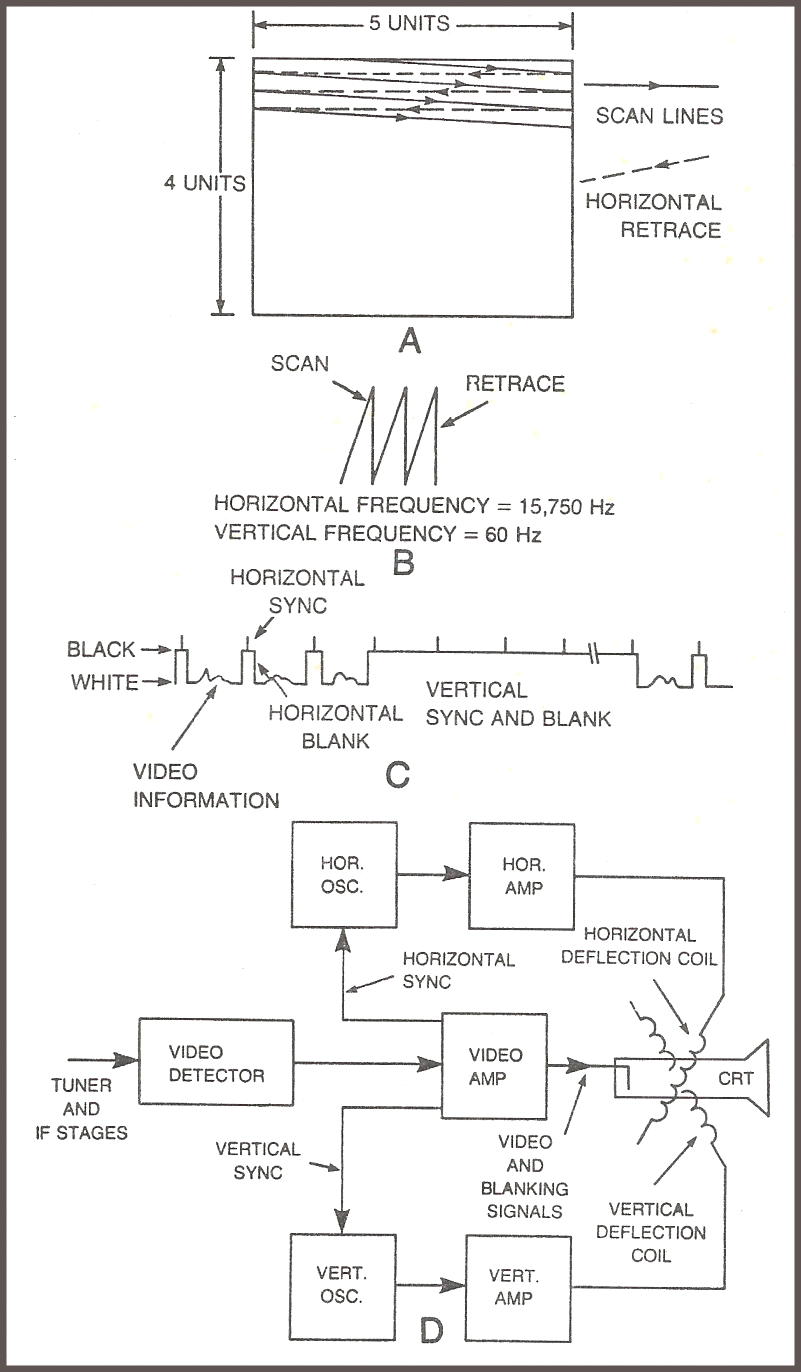
\includegraphics[width=0.95\textwidth]{images/fig1-1_clear}
  \caption{Generating the TV raster. (a) The basic raster as it appears on the screen. (b) The sawtooth waveform characteristic of horizontal and vertical raster scanning. (c) A composite video waveform. (d) TV receiver block diagram showing sections relevant to TV games.}
\end{figure}

The broad vertical sync and blanking pulse in Fig. 1.1c carries horizontal-sync pulses along its top. This is a feature that is necessary for maintaining horizontal sync during the relatively long vertical retrace time. Without maintaining horizontal sync during this time, the picture would tend to be torn out of sync in the upper left-hand corner of the screen, the place where the beam is located when it is no longer blanked.

The block diagram in Fig. 1.1d shows the portions of a TV receiver that are especially relevant to TV games. Horizontal- and vertical-sync pulses are taken from the video amplifier and are used for synchronizing their respective sawtooth oscillators. Once the sawtooth waveforms have been amplified, they are applied to sets of coils (the yoke) around the neck of the CRT. The magnetic fields thus generated are responsible for positioning the electron beam.

The actual video information and blanking signals are applied to the cathode of the CRT to modulate the brightness of the beam. The blanking pulses have a polarity that cuts off the beam completely. Lower voltages create varying degrees of gray and white. Referring to the composite video waveform in Fig. 1.1c, the “black” voltage levels are near the top, while the “whites” are near the bottom.

The video information, tucked between each horizontal-blanking pulse, thus creates shades of gray, the lower the voltage level, the whiter the spot on the screen.

This is hardly a complete description of the TV system, but it does touch upon those principles relevant to understanding the operation of TV games. Readers interested in more details about TV systems should consult a good TV textbook.

\newpage
\section{THE BASIC VIDEO GAME SYSTEM}

The whole point of the video game system is to create images on the screen that have shapes and motions relevant to a particular game scheme. These images, however, must be created in the context of a conventional TV system, and that means generating horizontal- and vertical-sync/blank pulses as well as game video information.

It turns out that the game system must be under the control of its sync pulses at all times, so it is important to have a reliable and accurate source of such pulses, not only for operating the game, but also for controlling the beam on the screen of a conventional TV receiver.

The whole game system is ultimately synchronized by a crystal oscillator. In this particular case, the oscillator runs at 14 MHz. The 14-MHz pulses from the oscillator operate a 9-bit binary counter that ultimately yields the 15,750-Hz pulses required for horizontal synchronization. During the counting interval, however, the horizontal-count circuit generates a distinctive pattern of binary numbers that actually indicate the horizontal position of the beam on the screen. See Fig. 1.2.

The 15,750-Hz output of the horizontal-counting circuit clocks yet another 9-bit binary counter, the vertical-count circuit. This circuit utlimately produces the necessary 60 Hz vertical-sync pulse, but in the meantime, it also generates a 9-bit binary code that indicates the vertical position of the beam on the screen.

In a manner of speaking, then, the TV game system always knows exactly where the beam is situated on the CRT screen. A pair of 9-bit binary numbers indicate the coordinates in a manner quite similar to the x, y coordinates of a conventional graphing scheme.

Since the game system knows where the beam is located at any given moment, it is possible to generate White or black video levels to create images on the CRT.

Notice in Fig. 1.2 that the sync pulses, blanking pulses, and game video information are combined to create the composite video signal. The only step remaining after that is to place the signal onto an rf carrier that will feed it through the tuner section of a conventional receiver. The rf modulator, incidentally, can be omitted from the system if the composite signal is applied directly to the video amplifier in the TV set. This calls for some surgery on the receiver circuitry, and many experimenters are unable or unwilling to do that sort of job.

\begin{sidewaysfigure}
  \centering
  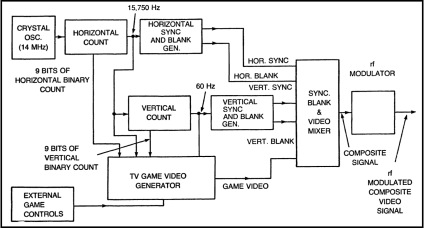
\includegraphics[width=0.95\textwidth]{images/fig1-2}
  \caption{The basic TV game system block diagram.}
\end{sidewaysfigure}

As far as this book is concerned, the bulk of the circuits blocked out in Fig. 1.2 is the same for every game. Only the game video generator and external game controls change. Most of the circuitry is thus built into a permanent unit called the Sourcebox unit. This particular part of the system is described in great detail in Chapter 2. The remainder of the book deals with experiments, examples, and design hints for the game video generator and external game controls, units that are plugged into the standard Sourcebox.


\section{HOW TO USE THIS BOOK}

This book leads the prospective TV game designer through a series of experiments, examples, and hints that are all intended to make game design possible and fun for just about anyone willing to make the effort. Generally speaking, the material (or “lessons,” if you will) are presented in order of importance. It would be difficult, for instance, to begin your study of TV games in the middle of the book, because each chapter assumes an understanding and some experience with the ideas presented in all the previous chapters.

Build up the systems one step at a time, performing the suggested experiments and trying some of your own. Hands-on experience is the key to designing games of your own, and the only way to get that kind of experience is by doing the work suggested here.


\section{LOCATING PARTS}

Most of the parts specified in this book are available from stores such as Radio Shack. In many instances, Radio Shack part numbers are specified for the benefit of experimenters who are not fully acquainted with other sources and substitution procedures.

Not all parts are available from Radio Shack, but it is not difficult to locate them from the many mail-order houses advertising surplus in newsstand electronics magazines.


\section{ASSEMBLING THE SYSTEMS}

There are few specific notes in this book concerning the final assembly of game circuits. It is left to the experimenter to devise clever assemblies of his or her own, thereby removing the limitations on fun and imagination that characterize commercially available TV game systems.

Of course this approach puts something of an extra burden on the beginner, but what better way to learn than by doing?


\chapter{The Sourcebox Unit}
 
The Sourcebox unit described in this chapter contains all the circuitry common to virtually all the TV games described in this book. It is the interface unit that stands between the game itself and the TV receiver. The Sourcebox unit, for instance, generates all the sync and blanking signals that synchronize both the TV raster and the game operations. Unless this system is built and made to operate properly, the experimenter cannot hope to make any real progress in his or her understanding of anything else that follows.

This chapter describes the theory of operation, shows complete circuit detail, and provides some practical hints on construction. The opening section of Chapter 2 gives the experimenter an opportunity to test the system.

The block diagram in Fig. 2-1 shows the basic circuits contained in the Sourcebox unit. The purpose of each block might be self-evident to anyone who has made a thorough study of the material in Chapter 1. The following sections of this chapter, however, describe the purpose and theory of each block in some detail. The construction hints are inserted at appropriate places in the discussion, rather than at the end of the chapter.

\section{SOURCEBOX ORGANIZATION}

\begin{sidewaysfigure}
  \centering
  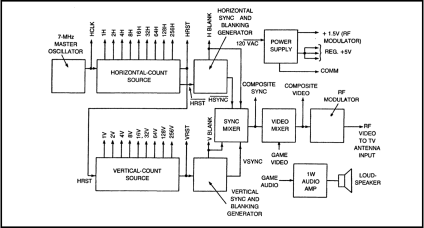
\includegraphics[width=0.95\textwidth]{images/fig2-1}
  \caption{Block diagram of the Sourcebox unit.
}
\end{sidewaysfigure}

The Sourcebox unit is organized into 10 basic circuits as described here:

\begin{enumerate}
\item \textbf{Power supply} — The power supply provides DC voltage levels to all of the circuits in the Sourcebox unit as well as plug-in game modules and the so-called tinkerboxes (breadboard units intended for se1f~learning experiments and game design). With the notable exception of the +1.5-V supply voltage for the rf modulator, the power supply gets its power from a standard 120-VAC, 60-Hz source.

\item \textbf{7-MHz oscillator} — This is the master clock oscillator for the entire TV game system. For best results, this should be a crystal-controlled, 14-MHz oscillator, followed by a toggling flip-flop that both divides the crystal frequency by two and assures a clean, 7-MHz HCLK waveform.

\item \textbf{Horizontal-count source} — The horizontal-count source generates a 9-bit binary counting code that divides the game screen into 455 equal horizontal segments. Each horizontal scan line on the screen is thus divided into 455 discrete sections, each of which is capable of rendering one bit of horizontal video information.

The nine binary-counting outputs are labeled 1H, 2H, 4H, 8H, and so on through 256H, with 1H being the least-significant (highest-frequency) output and 256H being the most-significant output bit.

The horizontal-count source also generates an HRST (Horizontal ReSeT) pulse that is used for clocking the vertical-count source and synchronizing the operation of some game circuits. An inverted version of this positive-going HRST pulse, designated \NOT{HRST}, is used for generating horizontal-sync pulses.

\item \textbf{Horizontal sync and blanking generator} — The inverted HRST pulse from the horizontal-count source is converted to horizontal sync and blanking pulses in this part of the Sourcebox unit. The horizontal-sync pulse (HSYNC) ultimately triggers the TVs horizontal retrace operation. The horizontal-blanking pulse (HBLANK) is likewise used for blanking horizontal retrace on the TV screen and for certain kinds of control operations for the video games.

\item \textbf{Vertical-count source} — The vertical-count circuit is almost identical to its horizontal counterpart. It generates a 9-bit binary count that divides the receiver’s raster into 262 vertical segments, or lines. In a manner of speaking, this circuit provides information regarding the position of the TV’s beam in the vertical sense.

Like the horizontal-count source, the nine outputs are labeled 1V through 256V, with 1V being the least significant bit. The circuit also generates a vertical-reset pulse (VRST) that is used for clocking the vertical sync and blanking generator as well as some of the game circuits.

\item \textbf{Vertical sync and blanking generator} — This circuit generates vertical sync and blanking pulses. The vertical-sync pulse ultimately initiates vertical retrace of the TV’s electron beam. The vertical-blanking pulse (VBLANK) is used for blanking the beam through vertical retrace and operating some of the game circuits.

\item \textbf{Sync mixer} — The sync mixer circuit combines the horizontal and vertical sync and blanking pulses to create a composite sync signal. This signal is practically identical to the sync signals from commercial TV stations. There is one important exception, however; this system does not have provisions for interlaced scanning. Few video games call for the higher degree of image resolution that characterizes commercial interlaced scanning.

\item \textbf{Video mixer} — The video mixer combines the sync and blanking pulses with game video information to provide a complete, composite video signal.

\item \textbf{RF modulator} — The rf modulator is responsible for amplitude modulating the composite Video signal with an rf frequency tuned to TV channels 2, 3, or 4. This part of the Sourcebox unit makes it possible to connect the game system to the VHF antenna terminals of any standard TV receiver.

NOTE: FCC REGULATIONS PROHIBIT CONNECTING THE OUTPUT OF ANY RF MODULATOR TO THE TERMINALS OF AN EXTERNAL ANTENNA. The antenna must be disconnected before the modulator is fixed to the TV receiver.

\item \textbf{Audio amplifier} — The audio for TV games is not carried via the composite TV signal through the receiver’s own audio system. Any audio special effects for a TV game are generated by the game system and merely amplified and reproduced by a small loudspeaker in the Sourcebox unit.
\end{enumerate}

\section{POWER SUPPLY}

\begin{sidewaysfigure}
  \centering
  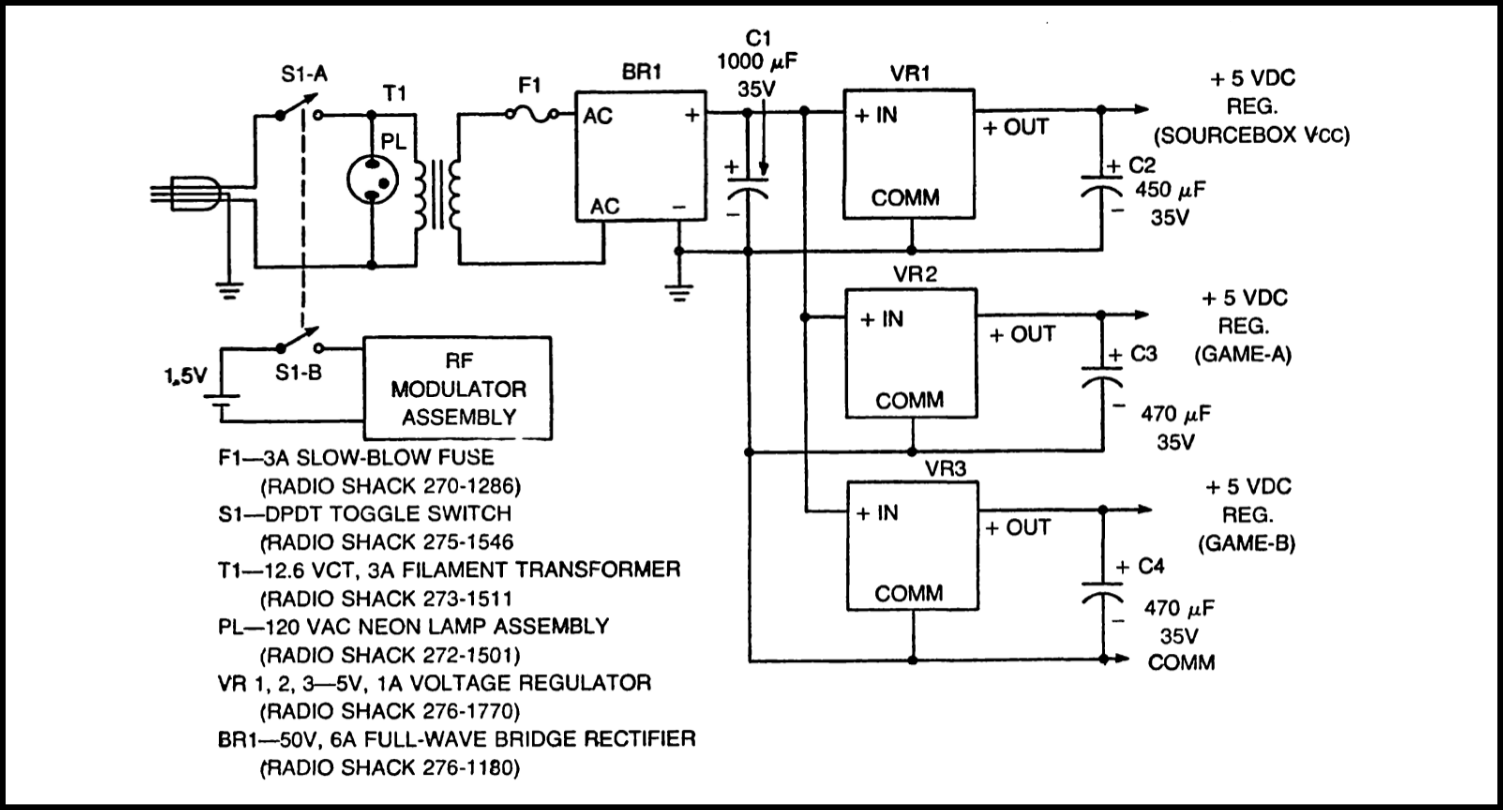
\includegraphics[width=0.95\textwidth]{images/fig2-2}
  \caption{Power supply schematic diagram.
}
\end{sidewaysfigure}

The power supply, illustrated in Fig. 2.2, services both the Sourcebox unit and external game circuits. This is a conventional IC power supply, taking its main power from the utility lines and converting it to an unregulated +18 VDC. Transformer T1 steps down the 120 VAC from the line cord to about 12.6 VAC at its secondary. The system is fused by F1, and then the lower AC voltage is rectified by a full-wave bridge rectifier assembly, BR1.

The +18-V peaks from the bridge circuit are then filtered to an unregulated 18 VDC by C1 before the voltage is applied to three +5-V, 1-A regulators, VR1 through VR3. The DC output from VR1 supplies its regulated 5-V level to circuits within the Sourcebox unit, including the audio amplifier. This particular +5-V source is also accessible to the outside for operating relatively low-power circuits.

The regulated outputs from VR2 and VR3 are used only for powering external game circuits and design breadboards. Some of the more involved video games described later in this book call for using all three voltage regulators to their maximum l-A capacity. In fact any experimenter contemplating designs for very elaborate games should count on constructing an outboard 5-V regulated supply capable of providing an additional one or two amps.

The rf modulator assembly, described in more detail later in this chapter, uses a separate 1.5-V AA battery as a power supply. Using a battery for this particular application ensures a clean, ripple-free modulated video waveform. For the sake of convenience, the battery supply for the rf modulator is switched on and off by means of the same toggle switch that applies 120 VAC to the 5-V power supply section.

The line cord is fed through the back of the Sourcebox housing, using a plastic strain relief (Radio Shack 278-1636) to prevent abrasion of the insulation and possible strain on the connections to the switch and power transformer.

Power switch S1 should be mounted at some convenient place on the front panel of the Sourcebox housing, preferably under the neon POWER ON indicator lamp.

Power transformer T1 should be mounted on the bottom, inside surface of the Sourcebox housing. The rectifier assembly, fuse and fuse holder, and all four filter capacitors can be mounted to a small perfboard or custom PC board. This compact power supply board can then be mounted near the power transformer, using insulated standoffs to prevent any short-circuit conditions to the Sourcebox housing.

\begin{figure}
  \centering
  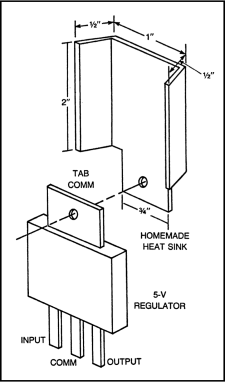
\includegraphics[width=0.95\textwidth]{images/fig2-3}
  \caption{Recommended heat sink for the voltage regulators.}
\end{figure}

The 5-V regulator assemblies tend to run a bit hot at times. To reduce the chances of destroying them by overheating, it is a good idea to mount them directly to the inside surface of the metal Sourcebox housing, or to affix a small heat sink to each of them. See the dimensions for one of the three heat sinks in Fig. 2-3. Similar heat sinks are available commercially, but it is rather easy to cut and bend custom versions from standard 1/16-in. aluminum stock.


\section{HORIZONTAL SOURCE BOARD}

\begin{sidewaysfigure}
    \centering
    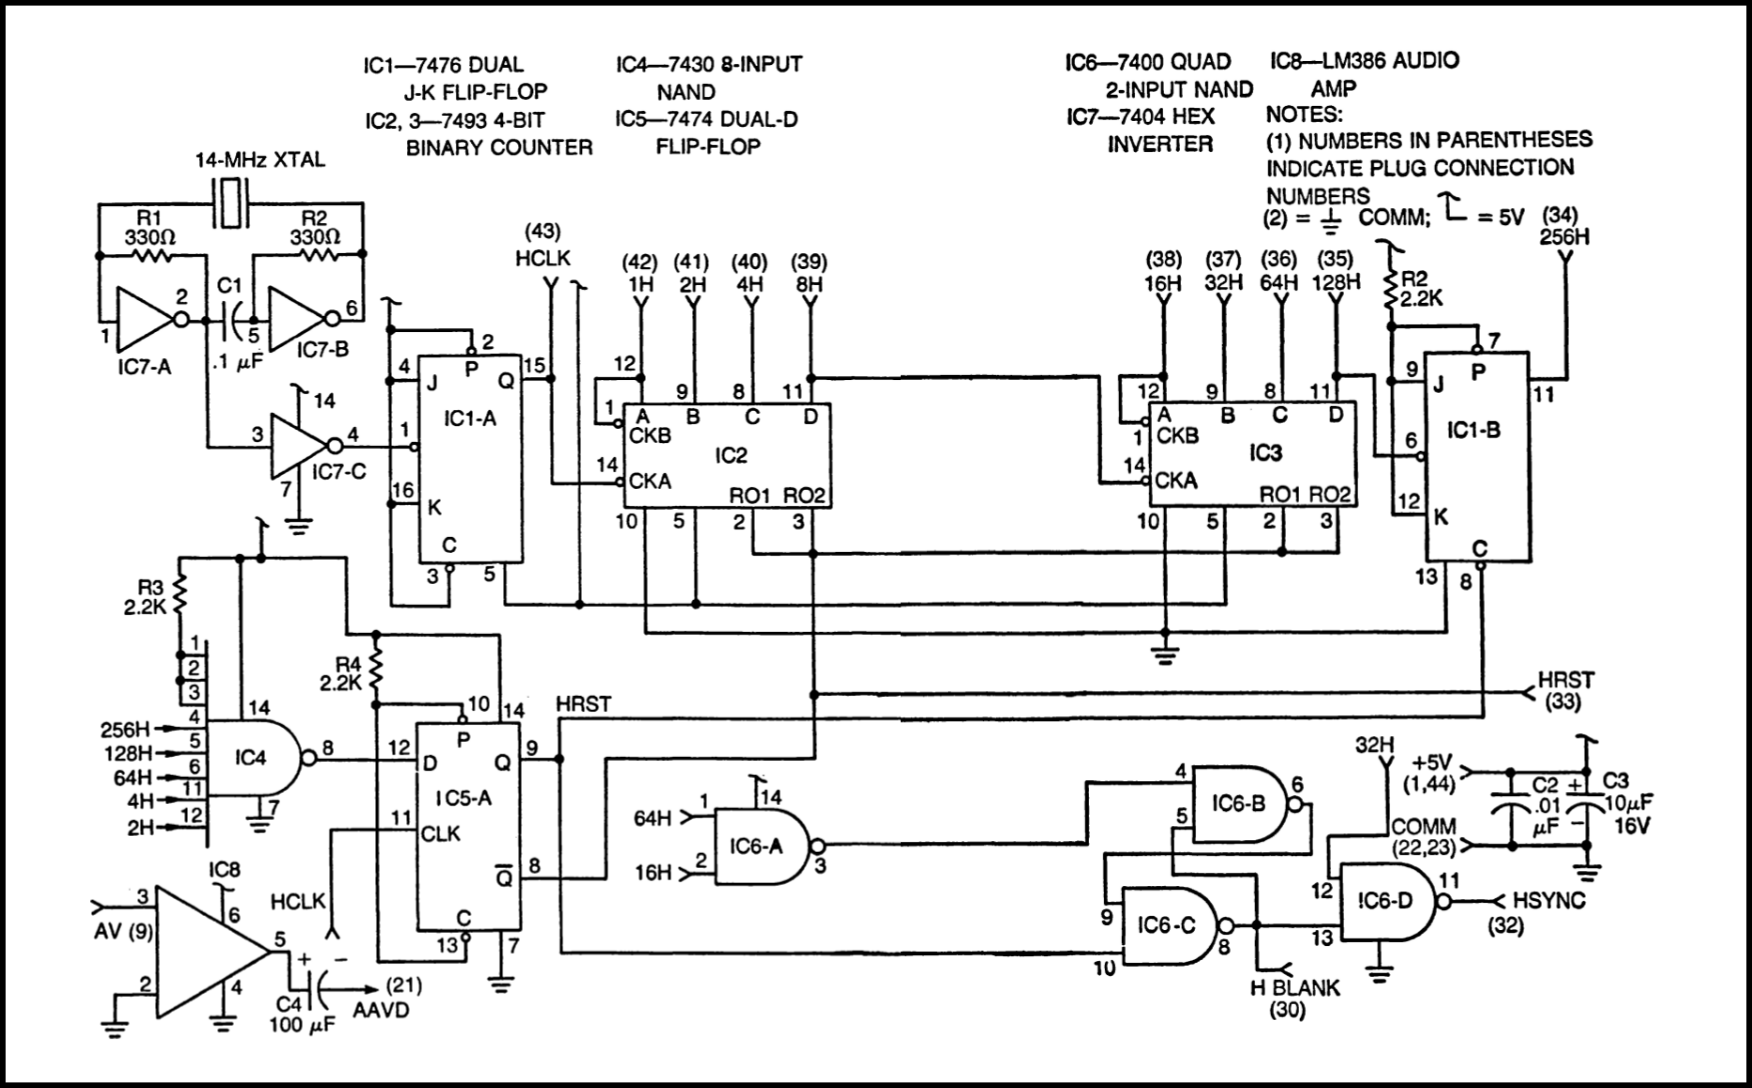
\includegraphics[width=0.95\textwidth]{images/fig2-4}
    \caption{Horizontal source board schematic diagram.}
\end{sidewaysfigure}

Figure 2.4 is a complete schematic diagram for the circuit that generates all the horizontal counting, sync, blanking, and reset pulses. This particular circuit board also holds the audio amplifier IC, not because the audio signal is part of the horizontal system, but because there is little space for putting it anywhere else in the Sourcebox unit.

The entire circuit can be mounted on a standard 44-pin, 4- by 4-inch card, such as a Radio Shack 276-153. In fact all of the circuits and systems described in this book can be built onto such a board and then plugged into the appropriate edge-card connector (Radio Shack 276-1551). The numbers in parentheses in Fig. 2.4 indicate card pin numbers arbitrarily assigned to the card-and-connector assembly.

The heart of the horizontal system, and indeed the video game as a whole, is the 14—MHz oscillator circuit. This little circuit is made up of a crystal cut to about 14 MHz and TTL digital inverters 1C7 -A and IC7-B. Actually the crystal should have a frequency rating as close as possible to 14.3 MHz, although the system will allow values within 2\% of 14.3 MHz. James Electronics supplies an ideal crystal for the job (14.31818 MHz). Order part number CY14A, James Electronics, 1021 Howard Ave., San Carlos, CA 94070.

Although the oscillator is basically a digital circuit, the waveforms from IC7-A and IC7—C appear sinusoidal on an oscilloscope. The toggled J-K flip-flop, ICl-A, isolates the oscillator from the rest of the circuitry and divides the 14. 3-MHz frequency by two. The output of ICl—A is thus a quasi-sinusoidal waveform having a frequency close to 7.015 MHZ. This is the system's HCLK signal.

1C2, 1C3, and ICl-B make up the 9-bit horizontal-count source. 1C2 and 1C3 are ordinary 4-bit binary up counters connected so that they generate an 8-bit binary count. IC1-B is a toggled J-K flip-flop that generates the 9th bit. Note that the outputs of these counters are labeled 1H through 256H, the labels used so frequently throughout this book.

The nine horizontal—count sources are connected directly to output terminals, but there is a selection of five of them that also go to the inputs of 1C4, an 8—input NAND gate. This is all part of a circuit that restricts the counting range of the horizontal—count source to 455 HCLK pulses. A 9-bit counter without this resetting circuit would count 511 states.

The resetting circuitry senses a count of 454 at IC4, generating a negative-going pulse at the D input of ICSA. IC5A is an edge-triggered D flip-flop which sets its Q output to the D-input logic level whenever its CLK input shows a positive-going edge. ICS-A is clocked by HCLK in this case; and as long as the horizontal—count source is generating numbers less than 454, the Q output of IC5-A remains at a logic-1 level. The complemented output from Q is at logic 0 at the same time.

One HCLK pulse after the count reaches 454, however, IC5—A loads its Q output with a logic-0 level and the Qoutput takes on a logic—1 level. This condition immediately clears all nine bits from the horizontal-count source to zero, thus restarting the 455«step operation all over again.

The signal from the Q output of IC5-A is thus a negative-going pulse that lasts for one HCLK pulse interval and occurs at the very beginning of each horizontal-count cycle. A positive- going version of that same pulse, HRST, is directed to 1C2, 1C3, and the plug assembly leading to the outside world.

The circuit build around the four Z-input NAND gates of 1C6 are responsible for generating the horizontal blanking (HBLANK) and inverted horizontal sync (HSYQLpulses. IC6-B and lC6-C make up what is commonly known as a R—S f lip-flop. Whenever the negative—going HRST pulse is directed to the pin—10 input of IC6-C, the output of that same 1C is set to a logic—1 level. The device remains in that state while the horizontal—count source is cleared and restarted. The moment the count reaches 80, as determined by the 16H and 64H inputs to IC6-A, this flip-flop circuit is reset so that the pin—8 output of IC6-C returns to logic 0. This point then remains at logic 0 until another HRSTpulse occurs.

The real significance of the output of IC6-C is that it generates the system’s HBLANK pulse, a positive pulse that begins as the horizontal-count circuit is reset to zero and ends 80 HCLK pulses later. Ultimately the beam on the TV screen will be blanked off through this 80-pulse, horizontal blanking interval.

The horizontal sync pulse is generated at IC6-D. This NAND gate is normally gated off by the logic-0 level from IC6-C. Whenever lC6—C is generating an HBLANK signal, however, IC6-D is open to the 32H signal at its pin-12 input. An inverted version of 32H thus appears at the output of IC6-D, but only through the horizontal blanking interval. See the waveforms in Fig. 2-5.

Looking at the HBLANK and HSYNC sequence in detail, the positive HBLAN K pulse begins first. Thirty-two clock pulses later, the inverted HSYNC pulse begins, lasting through count 64. HBLANK finally ends at count 80. The overall effect is a combination of horizontal blanking and sync pulses that work very much like their counterparts in a commercial TV broadcast signal.

The only purpose of audio amplifier 1C8 is to amplify any special—effects sounds and match the circuit to an 8-ohm loudspeaker. Since audio special effects are not described until Chapter 10, the volume control and loudspeaker need not be connected at this time.

% Fig. 25. Horizontal blanking and sync waveforms.

The volume control, speaker, and amplifier arrangement are shown in more detail in Fig. 2-6. Control R5 should be mounted on the front panel of the Sourcebox, while the loudspeaker can be positioned at any convenient place inside the box.

\section{VERTICAL SOURCE AND COMPOSITE VIDEO BOARD}

The circuit in Fig. 2-7 shows the complete schematic diagram for the vertical-count source and composite video generator. The vertical-count source consists of 1C1, 1C2, 1C3, IC4-A, and 1C5. The remainder of the circuit is responsible for composite video operations.

The vertical-count source is a 9-bit binary counter made up of two 4—bit counters and a toggled J -K flip-flop, 1C3. The natural counting range for a 9-bit counter is between 0 and 511; but like the horizontal-count generator, this circuit is fixed so that it counts a much more limited range.

Note that the two counters, 1C1 and 1C2, are cleared by the Q output of ICS, while the J -K flip-flop (1C3) is cleared to zero by the Q output of 1C5. 1C5 is a positive-edge triggered D flip-flop having a Q output that takes on the logic level of its D input whenever the CLK input shows a positive-going edge. The flip-flop in this case is clocked by HRST from the Horizontal Source board-at a frequency very close to 15,750 Hz.

NAND gate IC4-A keeps the D input to 1C5 pulled up to logic 1 most of the time, so the repeated HRST pulses at the CLK input keep the Q output of ICS fixed at logic 1 most of the time. There is a time, however, when the D input to 1C5 is set to logic 0: when the 1V, 4V and 256V inputs to IC4—A show logic 1 at the same time. This condition represents count 261 from the vertical-count source, and it is responsible for clearing the counters back to zero.

The vertical-count section thus generates 260 different patterns representing that many vertical lines on the screen.

The vertical-blanking and sync pulses are generated in a fashion almost identical to the corresponding horizontal section. One difference is that this circuit is built around a flip—flop triggered by positive-going, rather than negative-going, pulses.

The VBLANK generating flip-flop is composed of NOR gates IC6-A and IC6—B. The pin-4 output of IC6B is at logic 0 most of the time, rising to logic 1 only when a VRST (vertical reset) pulse occurs at the Qoutput of 1C5. This pulse sets the pin-4 output of IC6—B to logic 1 and, as described earlier in this section, clears the vertical-count source to zero.

The VBLANK signal remains at this logic-1 level until the 16 V signal at the input of IC6-B goes to logic 1. This action returns the pin-4 output of IC6-B to zero and, in fact, forces it to remain at 0 until another VRST pulse occurs.

The VBLAN K signal thus goes to logic 1 the instant the vertical counters are reset to zero, and it remains in that condition until the counters increment to count 16. VBLANK can then be described as a positive-going pulse that lasts 16 HRST pulses.

% Fig. 2-6. The complete audio amplifier system.
% Fig. 2-7. Vertica‘ source and composite video board schematic.
% Fig. 2-8. Vertical blanking and sync waveforms.

The vertical-sync pulse, VSYNC, is generated at IC4-B. This particular designation does not appear on the schematic, however, because it is never used alone anywhere else in the system.

IC4-B has an output that remains at logic 1 as long as VBLAN K is at 0. When VBLANK rises to logic 1, indicating it is time to blank the vertical retrace on the TV screen, IC4—B allows 4V and an inverted version of 8V to pass. The result at the output of IC4-B is a negative-going pulse that begins a count 4V and ends at 8V. This is the vertical-sync pulse. See the VBLANK and VSYNC pulses illustrated in Fig. 2-8.

The remaining circuitry in Fig. 2-7 is responsible for combining both the horizontal- and vertical—sync and blanking pulses, and then working the composite sync waveform together with the game video.

The horizontal— and vertical-sync pulses are effectively combined in the EXCLUSIVE-OR gate, IC7-A. The output of this gate, shown in Fig. 2-9(a), shows the 15, 7 50-Hz horizontal sync pulses in a positive-going, active-high format until the vertical-sync pulse occurs. At that moment, the horizontal pulses switch to an active-low format, providing the effect of a serrated vertical-sync pulse, an effect that is necessary for maintaining horizontal sync through vertical sync and retrace.

IC7-B serves merely as an inverter for obtaining an inverted version of this composite sync signal.

The horizontal— and vertical-blanking pulses are ORed together in IC9-C and IC9-D, and then these combined signals are ORed with the game video in ICQ-B. The output of IC9-B is thus a combination of horizontal— and vertical-blanking pulses and any game video applied from external circuitry to IC9—A.

These two sets of waveforms—the composite sync from 1C7 -B and video and blanking pulses—are finally amplitude modulated at the 3-state buffer, IC8-A. A precise analysis of this operation is left to experimenters who have some experience with Boolean algebra. The overall effect, however, is shown in Fig. 2-9(b).

The composite video waveform in Fig. 2-9(b) clearly shows three distinct voltage levels. The highest voltage level, about +5V, is the domain of the blacker-than-black sync pulses. At the other extreme is the white-video information, at about 0V. Black-video information and the blanking pulses fall between these two extremes, occuring only when the 3-state buffer is put into its high-impedance state by the output of IC6-D.

The vertical— count and composite-video board in Fig. 2-7 can be assembled on the same kind of 44-pin edge card that the horizontal section is. Both boards should be situated in their respective edge-card connectors in the Sourcebox housing.

% Fig. 2-9. Composite waveforms. (a) Composite sync. (b) Composite video to the modulator.
% Fig. 2-10. Suggested cabinet layout for the Sourcebox unit.

\section{THE RF MODULATOR}

The rf modulator is responsible for modulating the composite video (CVID) from the vertical/video board at a VHF frequency that can be selected on TV channels 2, 3, or 4. In a word, the whole idea is to get all this video, sync, and blanking information into a conventional TV receiver.

% Fig. 2-11. Listing of power suppIy terminais and signals that must be present at the interface plug.

It is possible to build VHF modulators from scratch, but considering the fact these little circuits are now commercially available for about \$10, the job of building one from scratch is hardly worth the trouble.

Suitable modulators are now being used by microprocessor enthusiasts who want to interface their computer systems with a TV display. 80 the best source of modulators is the amateur computer shops now springing up all over the country. At the time of this writing, Radio Shack is planning to offer a suitable modulator in the near future. Although it is intended specifically for use with that company’s microprocessor system, it would serve our purposes quite well.

Mount the modulator inside the Sourcebox unit, as far as possible from the master clock and crystal (to avoid possible rf interference between the two).

\section{SOME MECHANICAL CONSIDERATIONS}

All of the Sourcebox circuitry fits quite nicely into Radio Shack’s “compact” 57/s-by 9- by His-inch cabinet (Radio Shack 270-281). See Fig. 2-10.

The two major circuit boards can be inserted into 44-pin edge-card connectors mounted vertically on the inside rear surface of the cabinet. The rf modulator is likewise mounted on that surface, using a 2-terminal, feedthrough TV antenna connector (Radio Shack 274-663). The power supply components are mounted inside the cabinet as described earlier in this chapter.

What has not been adequately described thus far is the means for getting access to the horizontal- and vertical-counting signals as well as any other system inputs and outputs that are vital to the operation of game systems. The most convenient way to interface the Sourcebox with the outside world is by means of another 44-pin edge-card connector that feeds through the back of the cabinet.

All of the connections between the Sourcebox and outside world are made through this connector. Its solder connections are inside the cabinet, connected to the appropriate signal sources as suggested in Fig. 2-11. Getting access to these signals from the outside world is thus a simple matter of plugging the appropriate 4-by 4—inch 44-pin PC card into the plug on the back of the cabinet.

No matter how you choose to arrange the circuitry for the Sourcebox unit, bear in mind that you must have convenient access to the supply voltages and signal connections listed in Fig. 2-11.


\chapter{Building Static Figures}

For the purposes of this book, static figures are considered any figures, no matter how simple or complex, that do not move on the screen. Such figures, in the context of TV games, can represent game boundaries, obstacles and nonmoving targets.

A static figure, incidentally, does not have to be a visible one. Invisible figures can add an extra bit of challenge to an otherwise too-simple game; but more importantly, invisible lines and rectangles can serve as “windows” for confining other images to a field that is smaller than the TV screen.

Static figures, whether visible or not, play invaluable roles in TV-games technology; and it turns out that building static figures can be a fascinating and rewarding pastime in itself.

This chapter describes a number of basic techniques for build-ing static lines, bars, and rectangles, while the following chapter takes up the special subject of building complex static figures (circles, figures with diagonal lines, images of people, rocket ships, cars, etc.).

Each technique is illustrated with several specific examples, and the reader will find the procedures used many times and in many different ways throughout the book. It is important to bear in mind, however, that the purpose of this book is to provide some guidelines for creating original TV games and displays. For that reason, alone, it is just as important to understand the essence of each figure-building technique as it is to see how the specific examples work.

None of the figure-building techniques is really any better than the others under all possible circumstances. The most appropriate technique depends on the size, position, general configuration, complexity of the figure, and the role the figure is to play in the display.

The selection of a figure-building technique thus calls for an intelligent decision on the part of the experimenter, so it is important to stfidy this entire chapter and the one that follows before making a firm commitment to the circuit for an original TV-game display.

A prudent student of TV—game technology will breadboard the circuits as they are encountered in these chapters. Of course it takes longer to become acquainted with all the circuits this way, but this doing-whiIe-reading approach makes the learning process much easier, more effective, and a whole lot more fun. Try building the specific examples first, then test your understanding by attempting to create a few static images of your own.

\section{LINES AND BARS DIRECTLY FROM THE COUNT SOURCES}

One of the simplest and most straightforward ways to create simple lines and bars on the screen is by combining the waveforms already available from the Sourcebox unit. All of the horizontal-count outputs quite naturally generate alternate black and white vertical bars or lines on the screen, while the vertical-count outputs create horizontal bars.

Figure 3—1 summarizes five different horizontal— and vertical-count signals as they appear on the TV screen. To view the figures as shown here, simply connect a jumper wire between the designated horizontal- or vertical-count output and the GAME VID IN terminal on the Sourcebox unit. This procedure, incidentally, assumes the CVID and MOD terminals on the Sourcebox unit are jumpered together as described in the previous chapter.

Note that the 256H display shows a vertical black bar that almost reaches the center of the screen. This is a clear indication that the 256H signal is at logic 0 through the first half of each horizontal trace. (A logic-O video signal always creates a black area on the screen, and a logic-1 signal creates a white area).

The figure for 128H shows twice as many vertical bars as the 256H signal does. The reason is rather easy to understand: the 128H frequency is twice that of the 256H count source. And in a similar manner, each lower-order H output shows about twice as many bars as the one preceding it. Outputs 8H, 4H, 2H, and 1H are not shown here because the lines are too fine and closely spaced to make a meaningful picture in the book. Look at them on your own TV screen, however.

A figure for 256V is not shown here because it does not make a very interesting picture. It is at logic 0 through all but the last four lines of the display. Figure 3-1 does show what you should expect to see from 128V, 64V, 32V, and 16V.

While inspecting these figures for yourself, take careful note of the fact that the bars for 64H and 64V are very close to the same size. The same is true for 32H and 32V, 16H and 16V, etc. From 64H and 64V downward, the lines are about the same size when comparing an H output with its vertical counterpart.

There is, however, an obvious difference between the sizes of the bars for 128H and 128V, and 256H and 256V. Keep these facts in mind for a time when you will be considering your own figure-building procedures.

An experimenter can be justifiably proud of his system when seeing these basic horizontal— and vertical—count bars for the first time. A lot of work and money has gone into building the Sourcebox, and this is the first solid result of all that work. But looking at these bars and lines can become rather boring after a while. So now it is time to begin using these lines and bars as mere building blocks for creating more-useful and interesting figures.

\section{THE LINE/BAR TINKERBOX}

Figure 3—2 shows a schematic diagram, physical layout, and parts list for a breadboard system we shall call the Line/ Bar Tinker-box. It is simply a selection of ICs that are most useful for creating certain lines and bars at desired positions on the screen. The main purpose of this Tinkerbox is to let the experimenter find out exactly what IC devices are necessary for building a desired line or bar on the screen. After taking careful note of how it is done with the Tinkerbox, the experimenter can transfer the ideas to a permanent cirucit.

The ICs are plugged into a standard breadboard and bus-strip assembly. (See the parts list in Fig. 3—2 for catalog numbers.) The breadboard assembly is connected to the Sourcebox unit via a multiconductor cable or bundle of wires. These wires are connected to the Sourcebox output connector by means of a standard 22-pin edge-card PC board. Figure 3-3 shows a connection diagram that corresponds with the Sourcebox output terminal configuration described in Chapter 2.

% Fig. 3-1. Video images available directly from the horizontal and vertical‘count sources.

To get a feeling for what the Tinkerbox can do and how to use it, connect the circuit shown in Fig. 8—4a. In this case, 256H is connected to pin 1 of 1C3, the 8-input NAND gate. If a test jumper is connected from that input point and the GAME VID IN terminal on the Sourcebox, the screen will show the usual 256H pattern.

But once that same signal passes through the NAND gate, the blacks and whites are reversed. In digital terms, a NAND gate with a single input works like a logic inverter—it reverses the logic-1 and -0 levels.

The signal from the NAND gate is then passed through an inverter circuit where the waveform is reversed once again. This operation brings the signal back to its original phase, thus creating an image on the screen that is in all respects the same as that created by the original 256H waveform.

Any horizontal- or vertical-count waveform can be applied to the input of the circuit in Fig. 3—43, and emerge in its original form from the output of the inverter circuit, ICl—A.

% Fig. 3-2. Most-used ICs for the Line/Bar Tinkerbox assembly. Other useful IC’s include a 7486 quad EXCLUSIVE-OR and a 7402 quad 2-input NOR gate.

So what is accomplished by the simple circuit in Fig. 3-4a? Not much in terms of building images for TV games. But the circuit does clearly demonstrate two important facts: a NAND gate inverts logic levels (and hence reverses blacks and whites), and doubly inverting a signal returns it ot its original phase.

% Fig. 3-3. Signal and power supply connections between the Sourcebox unit and Tinkerbox assembly. Note that the Sourcebox MOD and CVID terminals are connected together at the Tinkerbox.

Now wire the circuit in Fig. 3-4b. There are two inputs in this instance. The waveform from 256H is applied to an inverter circuit and then to one input of the 8—input NAND gate. The other input, 128H, goes directly to a second input of the NAND gate. The little screen figures accompanying the diagram in Fig. 3-4b show the patterns appearing on the TV screen as GAME VID IN is connected to various test points.

The essential point to note in Fig. 3-4 is the fact that thegutput figure shows a white bar only where the white bars for 256H and 128H overlap. In digital logic terminology, this circuit ANDs together the two signals appearing at the input of the NAND gate.

It is impossible to build the single white bar generated as the output of this circuit from any one horizontal-count output.

What would happen if both inputs are inverted before applying them to the NAND gate? Figure 3—4c demonstrates the answer to that question. The NAND gate does the same job as before, but now the whites for '2'5—613 and 128H overlap only at the right-hand edge of the screen.

Play with this basic idea, using various combinations of inverted and noninverted H inputs to the NAND gate. You might be puzzled with some of the results at this point, but the exact procedures for generating a vertical line at one desired place on the screen are outlined in great detail later in this section.

Incidentally, if you happen to stumble across some patterns that look especially useful or interesting for later work, take careful note of the circuit connections. Keep the results recorded in a notebook for future reference.

Figure 3-5 shows some similar tricks with the vertical-count signals. In Fig. 3-5a, the inputs are 128V and 64V; and as in the case of the horizontal demonstrations, the overall result is a white bar appearing at the location where the white bars at the inputs overlap.

White playing with various combinations of V signals, remember that 256V is not a very useful or interesting waveform. An inverted version of the 256V signal has little noticeable effect on these demonstrations, while a noninverted version applied to the input of the NAND gate blanks out just about all the useful working area of the screen.

The Tinkerbox, as described to this point, can be the source of a whole evenings entertainment for you. Your family and friends might not be overly impressed with the results at this time, but as long as you are having fun with the system and learning things as you progress, that is all that really counts.

% Fig. 3-4. Some vertical lines and bars from the Tinkerbox assembly. (a) A twice-inverted 256H signal yields a 256H pattern on the screen. (b) A NAND gate followed by an inverter combine two different horizontal-count signals such that the resultant is a white area where two white areas of the original signals overlap. (c) Another example of creating a moderately narrow, vertical white bar where two input signals have overlapping white areas.

The NAND gate, followed by an inverter circuit, performs an essential operation as far as building static figures is concerned. In the first place, you have already seen that this circuit yields an output that shows a white bar wherever the white bars at the input of the NAND gate overlap. And now it is time to study a second essential feature of this NAND/invert combination.

Any black or white bar from one of the basic horizontal— or vertical-count sources is always divided equally by a black/white alternation of the next-lower-order signal. Although this might seem to be a rather obscure fact at the moment, it is important you understand it thoroughly. So try an example with your Tinkerbox arrangement.

Feed 3 256H signal to the input of the NAND gate and note the signal on the TV screen as generated at the output of the inverter. It should be the now-fannliar 256H vertical pattern: a black space turning to white just left of center. Now apply the next lower-order H signal, 128H, to a second input of the inverter. That new waveform should cut the 256H pattern in half. It divides the white portion of 256H into equal-sized black and white—black first, then White.

This demonstrates the fact that any basic horizontal- or vertical-count display has its white section(s) cut in half by a black/ white alternation of the next-lower-count input. The black section of 256H is, incidentally, being cut in two also. But since this particular NAND/invert combination yields only overlapping white areas, the division of the black section cannot be seen on the screen.

To check your understanding of this principle, what do you suppose will happen when you add a third input, specifically 64H, to the NAND gate circuit? If 256H and 128H are already there, the 64H input should cut the white area of 128H in half—black first, then white.

The next-lower-order H signal is 32H; and if it is included as a fourth input to the NAND gate, it cuts the bar in half again. This procedure can continue until all eight inputs on the N AN D gate are used.

While running this experiment, notice that the white bar on the screen seems to grow narrower as each input is added. Furthermore, it is narrowing from the left-hand side. The right-hand side is remaining fixed. Bear this effect in mind while considering the next set of experiments.

Remove all inputs to the 8—input NAND gate except 256 H. The image on the screen should then be the standard black-to-white 256H signal. Apply the 128H signal again, but run it through an 


% Fig 3- 5. Some horizontal lines and bars from the vertical— count sources. (a) A wide white bar at the bottom of the screen representing the area where white areas ot128V and 64V overlap. (b) Building a broad, horizontal bar Iust below the center of the screen inverter first. The inputs to the N AN D gate are now 256H and 128H. How has this inversion of the 1281-1 signal influenced the pattern on the screen?

The white portion of the 256H signal is cut in two by a white/black alternation this time. Recall that connecting a noninverted version of 128H to the NAND gate also cut the white portion of the 256H image in two, but with a black-to-white alternation.

Continue adding inverted versions of the H-count signals to the NAND gate until all eight inputs are used. If you are adding these inputs in decreasing order—from 128H to 64H, to 32H, to 16H, etc. —you will see that the white bar on the screen narrows in from the right-hand side.

As far as the line-building effect on the TV screen is concerned, adding a noninverted version of the next-lower-order H input nar... 

\end{document}
